\documentclass{report}
\usepackage{ugentstyle}

\begin{document}
	\maketitle{Beveiliging van netwerken en computers}
	\tableofcontents
	\chapter{Basisconcepten}
	Computerbeveiliging 
	
	\chapter{Netwerk en communicatiebeveiliging}
	Voorlopig hebben we enkel de basisconcepten gezien zoals: symmetrische encryptie, asymmetrische encryptie, hashfuncties en message authentication codes. Dit hoofdstuk zal deze concepten toepassen om beveiligingsprotocollen te ontwikkelen voor netwerken.
	\section{SSH}
	SSH (Secure Shell) is een \textbf{applicatielaagprotocol}. Ondanks deze naamgeving bevat SSH ook een \textbf{transportlaagprotocol}, met als bedoeling een veilige connectie te maken tussen andere OSI applicatielaagprotocollen (bv HTTP) en de werkelijke OSI transportlaag. SSH can draaien op zowel workstations als routers en switches. Routers en switches volgen de OSI laag namelijk niet strict, zodat zij ook een applicatielaag hebben. Vroeger werd het programma \textbf{telnet} gebruikt om remote configuratie toe te passen. Deze manier van werken is \textbf{onveilig} aangezien verkeer tussen de local host en remote host niet geëncrypteerd wordt, zodat deze door eender wie kunnen bekeken worden. SSH verhelpt dit probleem door de informatie te encrypteren. Vrijwel alle UNIX en Linux distributies komen met een versie van SSH geinstalleerd. SSH laat onder andere toe om:
	\begin{itemize}
		\item een veilige remote verbinding op te zetten vanuit eender welke local host naar eender welke remote host. Het protocol maakt gebruik van erkende algoritme voor zowel encryptie (sleutels van ten minste 128 bits), data-integriteit, sleuteluitwisselingen en public key management. Tijdens het leggen van een connectie worden algoritmen tussen de local host en remote host afgesproken, op basis van welke ze al dan niet ondersteunen,
		\item TCP te tunnelen via een SSH connectie,
		\item bestanden te verplaatsen, gebruik makend van bijhorende protocols zoals SCP (Secure Copy) of SFTP (SSH File Transfer Protocol),
		\item zowel X-sessions als poorten te forwarden.
	\end{itemize}
	\subsection{Architectuur}
	SSH kan opgesplitst worden in drie elementen: Transport Layer Protocol, User Authentication Protocol en het Connection Protocol.
	\subsubsection{Transport Layer Protocol}
	Dit protocol heeft onder andere de verantwoordelijkheid om: authenticeren van servers, sleuteluitwisselingen en perfect forward privacy implementeren. Perfect forward privacy wil zeggen dat, indien een sleutel gecomprimeerd wordt tijdens een sessie, deze geen invloed kan hebben op de beveiliging van vorige sessies. Dit protocol loopt uiteraard op de transportlaag, en in de meeste gevallen zal dit TCP zijn. Vooraleer de cliënt kan connecteren moet hij de \textbf{public host key} van de server bezitten. Hiervoor kunnen er twee modellen gebruikt worden (\accentuate{cfr. RFC 4521}) waarbij: 
	\begin{enumerate}
		\item de cliënt een lokale databank bevat die de mapping beschrijft van elke hostnaam naar de correspondeerde public host key. Op deze manier is er geen centrale entiteit nodig, maar het beheer van deze databank kan, indien deze groot genoeg wordt, lastig zijn om te onderhouden.
		\item de mapping bevestigd wordt door een \textbf{CA (Certification Authority)}. De cliënt kent in dit geval enkel de CA root key waarmee de geldigheid van elke host key kan nagaan die getekend zijn door deze CA. In dit geval moet de cliënt slechts één of enkele CA root keys bevatten. 
	\end{enumerate}
	Wanneer er een connectie kan gelegd worden van een cliënt tussen een server, is het eerste proces altijd het \textbf{onderhandelen van de algoritmen}. Deze stap zal algoritmen selecteren die compatibel zijn met zowel de cliënt als de server. Wanneer de cliënt een TCP connectie heeft met de server worden volgende pakketten verstuurd:
	\begin{itemize}
		\item \textbf{Identification string exchange.} Dit is een string dat zowel het protocolversie als de softwareversie van SSH bevat. Deze string wordt ten eerste van de cliënt naar de server verstuurd, waarop de server dan antwoord met zijn protocol en softwareversie. Indien hieruit blijkt dat de machines niet compatibel zijn met elkaar, wordt de connectie onderbroken \accentuate{(SSH2 is bv niet compatibel met SSH)} en worden volgend stappen bijgevolg niet meer uitgevoerd.
		\item \textbf{Algorithm Negotiation.} In deze fase sturen zowel de server als de cliënt een \\ \texttt{SSH\_MSG\_KEXINIT} bericht, die een lijst van alle ondersteunde algoritmen bevat, in volgorde van voorkeur. Elk type van algoritme zoals sleuteluitwisseling, encryptie, MAC algoritme en compressiealgoritme heeft zo zijn eigen lijst. Elk type moet dan ook een algoritme toegekend krijgen en wordt bepaald door het eerste algoritme dat de cliënt goed vind dat ook beschikbaar is op de server.
		\item \textbf{Key Exchange.} Indien de vorige fase goed gelukt is, start nu de sleuteluitwisseling. Voor de sleuteluitwisseling worden er momenteel slechts twee versie van \textbf{Diffie-Helman} ondersteund \accentuate{(cfr. RFC 2409)}. Het einde van de sleuteluitwisseling wordt gesignaleerd door een \texttt{SSH\_MSG\_NEWKEYS} pakket, met als gevolg dat zowel de cliënt als de server de gegenereerde sleutels mag gebruiken.  
		\item \textbf{Service Request.} De laatste stap, dat eigenlijk het begin is van een volgend proces, wordt gesignaleerd door een \texttt{SSH\_MSH\_SERVICE\_REQUEST} pakket. Dit pakket vraagt ofwel de start van het User Authentication Protocol of van het Connection Protocol. Alle verkeer tussen server en cliënt wordt op dit moment getransporteerd als de payload van een SSH Transport Layer pakket, beveiligd met encryptie en een MAC.
	\end{itemize}
	Een SSH Transport Layer pakket heeft de volgende vorm, waarbij elementen met een $\delta$-symbool geëncrypteerd en geauthenticeerd zijn en elementen met een $\Delta$-symbool ook optioneel gecompresseerd kunnen zijn:
	\begin{itemize}
		\item[$\delta$] \textbf{Pakketlengte (4 bytes).} De lengte van het pakket in bytes, zonder de lengte van de pakketlengte zelf en het MAC veld in beschouwing te nemen.
		\item[$\delta$] \textbf{Paddinglengte (1 byte).} Dit is de lengte van het random padding veld.
		\item[$\Delta$] \textbf{Payload}. De eigenlijke informatie van het pakket.
		\item[$\delta$] \textbf{Random padding.} Dit veld dient om cryptoanalyse moeilijk te maken. Kleine pakketten zijn op deze manier minder veel minder voorspelbaar en algoritmen, die vaak een kenmerkende vaste lengte hebben, worden ook moeilijker te achterhalen.
		\item[/] \textbf{MAC veld.} Dit veld wordt enkel gegenereerd indien dit zo in de onderhandeling besproken werd. Dit veld wordt berekent over het hele pakket en krijgt ook nog een bijhorend sequentienummer. Het sequentienummer start op 0, en wordt telkens met 1 geïncrementeerd voor elk pakket. Een aanvaller kan dit sequentienummer niet achterhalen aangezien een MAC een onomkeerbaar proces is.
	\end{itemize}
	\todo{juiste afbeelding}
	\begin{bytefield}[bitwidth = 1.5em, leftcurly = .]{16}
		\bitheader[endianness = big]{0 - 15} \\
		\begin{leftwordgroup}{packet}
			\bitbox{8}{pakketlengte}
		\end{leftwordgroup}
	\end{bytefield}

	Het \textbf{sleuteluitwisselingsproces} vraagt wat enige uitleg, er is echter nog niet nagegaan of deze sleutels op een \textbf{veilige} manier uitgewisseld worden. Op het moment van sleuteluitwisseling is er helemaal nog geen SSH connectie. Het uitwisselingsproces verloopt in twee fasen: eerst wordt er een gedeelde sleutel gegenereerd met Diffie-Helman, daarna wordt deze gedeelde sleutel gesigneerd met de publieke sleutel van de cliënt voor authenticatie. Sleutels kunnen ook heruitwisseld worden, hierbij gelden volgende regels:
	\begin{itemize}
		\item Mogelijk op elk moment, behalve tijdens het sleuteluitwisselingsproces.
		\item Kan aangevraagd worden door beide partijen.
		\item Sessie identificaties blijven ongewijzigd.
		\item Cryptografische algoritmen kunnen gewijzigd worden.
		\item Sessiesleutels worden vervangen.
	\end{itemize}
	Meestal worden sleutels vervangen na het behalen van een bepaalde quota zoals een tijdslimiet of het aantal totaal verstuurde bytes.
	\subsubsection{User Authentication Protocol}
	Dit protocol specifieerd \textbf{hoe} een cliënt zich moet authenticeren aan een server. Meerdere methoden zijn mogelijk waaronder de drie belangrijkste ervan: Public Key Authentication, Password Authentication en Host Based Authentication:
	\begin{itemize}
		\item \textbf{Public Key Authentication.} De implementatie van deze methode is afhankelijk van het gebruikte public-key algoritme. Een cliënt verstuurt berichten, dat gesigneerd is door de cliënt zijn private sleutel, naar de server, die de publieke sleutel van de cliënt bevat. De server gaat na of deze publieke sleutel nog geldig is en zoja, of dat de signatuur correct is. 
		\item \textbf{Password Based Authentication.} De cliënt verstuurt zijn paswoord, dat geëncrypteerd wordt door het SSH Transport Layer Protocol naar de server, die nagaat of het paswoord correct is.
		\item \textbf{Host Based Authentication.} De authenticatie is gebaseerd op de host in plaats van een individuele gebruiker (cliënt) zelf. De cliënt verstuurt een handtekening, gemaakt met de private key van de host. De server verifieerd enkel de host, en dus niet de individuele gebruikers. 
	\end{itemize}

	\subsubsection{Connection Protocol}
	Het connection protocol veronderstelt dat een beveiligide, geauthenticeerde verbinding tot stand gebracht is. Deze verbinding, \textbf{tunnel} genoemd, wordt gebruikt door het connection protocol om een aantal logische kanalen te multiplexen doorheen deze tunnel. Het connection protocol specifieert vier kanalen:
	\begin{enumerate}
		\item \textbf{Session.} Dit kanaal refereert naar het remote uitvoeren van een programma zoals een shell, een applicatie zoals e-mail of een systeemcommando. 
		\item \textbf{X11.} Het X Window System laat toe om applicaties te runnen op een server, maar dat ze eigenlijk op een desktop getoond worden.
		\item \textbf{Direct-tcpip.} Dit kanaal dient voor local port forwarding.
		\item \textbf{forwarded-tcpip.} Dit kanaal dient voor remote port forwarding.
	\end{enumerate}
	De lifecycle van een kanaal verloopt in drie stages: een kanaal openen, uitwisselen van informatie en een kanaal sluiten. Wanneer de server of de cliënt (hier uitgewerkt voor de cliënt) een kanaal wil openen, wordt er een lokaal nummer bijgehouden voor dat kanaal en wordt er een bericht verstuurt naar de server met volgende informatie: 
	\begin{itemize}
		\item Eén van de vier kanaaltypes. 
		\item Het lokale kanaalnummer van de cliënt.
		\item De initiële window size. Dit is het aantal bytes dat kan verstuurt worden naar de verzender zonder dat het venster moet aangepast worden.
		\item De maximum pakketgrootte specifieert hoeveel bytes een individueel pakket mag bevatten.
	\end{itemize}
	Als de server het kanaal kan openen, zal het een \texttt{SSH\_MSG\_CHANNEL\_OPEN\_CONFIRMATION} bericht versturen. Dit bericht bevat het kanaalnummer van de cliënt, het kanaalnummer van de server, en de waarde voor de window-en pakketgrootten voor inkomend verkeer. Als de server het kanaal niet kan openen, zal het een \texttt{SSH\_MSG\_CHANNEL\_OPEN\_FAILURE} versturen, met een foutmelding. Bij een open kanaal worden er voortdurend \texttt{SSG\_MSG\_CHANNEL\_DATA} berichten verstuurd, die het kanaalnummer van de ontvanger en een datablok bevat. Deze berichten kunnen in twee richtingen voorkomen. Tot slot kan er nog een \texttt{SSH\_MSG\_CHANNEL\_CLOSE} bericht verstuurd worden, die het kanaalnumer bevat dat gesloten moet worden.
	
	\subsection{Port forwarding}
	Port forwarding of port mapping is een toepassing van \textbf{NAT (Network Address Translation)} dat een een communicatieaanvraag van een specifiek adres en poort naar een ander zal omleiden. Op deze manier kan elke onveilige TCP verbindingen in een veilige SSH verbinding gemaakt worden. Een klein woordje uitleg over een poort. Een poort is een identificatie van een TCP-gebruiker. Elke applicatie dat bovenop TCP draait, heeft een poortnummer. Het \textbf{SMTP (Simple Mail Transfer Protocol)} luistert algemeen naar poort 25. Inkomende SMTP berichten zullen dus deze poortnummer bevatten. TCP Herkent dit poortnummer en zal het verkeer routen naar de SMTP server applicatie. SSH ondersteunt twee types port forwarding: local forwarding en remote forwarding:
	\begin{itemize}
		\item {Local forwarding.}
		\item {Remote forwarding.}
	\end{itemize}

	\section{Sleuteluitwisselingen}
	Gegeven twee partijen $A$ en $B$. Een sleuteluitwisseling kan op verschillende manieren gebeuren:
	\begin{enumerate}
		\item $A$ kan het fysiek afleveren aan $B$.
		\item Een betrouwbare partij geeft de sleutel fysiek aan $A$ en $B$.
		\item Als $A$ en $B$ vroeger al gecommuniceerd hebben, kunnen ze de vorige sleutel gebruiken om de nieuwe te encrypteren.
		\item Als $A$ en $B$ een beveiligide verbinding hebben met een derde partij $C$, dan kan $C$ de sleutel doorverwijzen naar $A$ en $B$.
	\end{enumerate}
	\subsection{Out-of-band sleuteluitwisseling}
	Sleutels niet-digitaal uitwisselen wordt out-of-band sleuteluitwisseling genoemd. Dit is toelaatbaar voor kleine organisaties maar voor grotere organisaties is dit niet voldoende.
	\subsection{Diffie-Hellman}
	Dit protocol was de eerste praktische methode om een gedeelde sleutel over een onbeveiligide verbinding te versturen, gebaseerd op discrete logaritmen. Het maakt gebruik van de eigenschap
	$$(g^b\;mod\;p)^a\;mod\;p = (g^a\;mod\;p)^b\;mod\;p$$ indien $p$ een priemgetal en $g$ de primitieve wortel modula $p$ is. Een voorbeeld is $p = 7$ en $g = 3$. 
	\begin{equation*}
		\begin{split}
			3^1 = 3 & = 3\;\hbox{mod}\;7\\
			3^2 = 9 & = 2\;\hbox{mod}\;7\\
			3^3 = 27 & = 6\;\hbox{mod}\;7\\
			3^4 = 81 &  = 4\;\hbox{mod}\;7\\
			3^5 = 243  & = 5\;\hbox{mod}\;7\\
			3^6 = 729  & = 1\;\hbox{mod}\;7\\
		\end{split}
	\end{equation*}
	Het algoritme verloopt in volgende stappen:
	\begin{enumerate}
		\item Alice en Bob zoeken een priemgetal $p$, en een daarbijhorende primitieve wortel $g$. Deze $p$ en $g$ mogen publiek gekend zijn.
		\item Alice kiest een geheim getal $a < p$. Haar publieke sleutel is $y_A = g^a\;\hbox{mod}\;p$.
		\item Bob kiest een geheim getal $b < p$. Zijn publieke sleutel is $y_B = g^b\;\hbox{mod}\;p$.
		\item Alice en Bob bereken respectievelijk $y_B^a\;\hbox{mod}\;p$ en $y_A^b\;\hbox{mod}\;p$. Deze zullen beiden dezelfde uitkomst bekomen, en wordt dan hun sleutel. 
	\end{enumerate}
	 Aangezien $g^x$ elk mogelijk getal zal genereren modulo $p$ voor alle $x < p$, is het moeilijk voor een aanvaller, die de publieke sleutels toch kent, de geheime sleutel te achterhalen. Ze moeten hierbij het discrete logaritme probleem oplossen. 
	 
	 Stel $p = 23$ en $g = 5$. Alice neemt $a = 6$ en Bob neemt $b = 15$, dan wordt $y_A = 5^6\;\hbox{mod}\;23 = 8$ en $y_B = 5^{15}\;\hbox{mod}\;23 = 19$. Alice berekent $19^6\;\hbox{mod}\;23 = 2$ en Bob berekent  $8^{15}\;\hbox{mod}\;23 = 2$.

	 Normaal wordt $p$ een priemgetal van ongeveer 300 cijfers genomen. De getallen $a$ en $b$ zijn dan weer minstens 100 cijfers lang. De geheime sleutel bepalen, indien $g$, $p$, $y_A$ en $y_B$ gekend zijn duurt quasi oneindig lang. 

	\subsubsection{Nadelen Diffie-Hellman}

	\subsection{Sleuteldistributiecentrum}
	Het sleuteldistributiecentrum vermijdt dat gebruikers zelf de sleutel moeten overhandigen. Elke gebruiker heeft een geheime sleutel die kan gebruikt worden om met het \textbf{KDC (Key Distribution Centre)} te communiceren. Er zijn twee soorten sleutels: de sessiesleutels zijn een tijdelijke sleutel die gebruikt worden voor één enkele sessie. Deze sessiesleutel wordt gebruikt om data te encrypteren tussen verschillende gebruikers. De ander sleutel is de mastersleutel. Deze wordt gebruikt om sessiesleutels te encrypteren en wordt gedeeld tussen een gebruiker en de KDC. De basiswerking van de KDC (figuur \ref{fig:basiswerkingKDC}) is als volgt:
	\begin{enumerate}
		\item Alice vraagt aan de KDC om een verbinding op te zetten met Bob. Alice stuurt ook een "nonce" $N_1$. Dit is een willekeurig getal dat slechts éénmaal gebruikt wordt om replay aanvallen te voorkomen.
		\item De KDC geeft volgende informatie terug, dat geëncrypteerd wordt door Alice haar sleutel $K_{A-KDC}$: De sessiesleutel, de identiteit van Bob, dezelfde nonce dat Alice stuurde naar de KDC, en geëncrypteerde data (met Bob zijn sleutel $K_{B-KDC}$).
		\item Alice verstuurt de geëncrypteerde data naar Bob.
		\item Bob antwoordt met een tweede nonce $N_2$, geëncrypteerd met de sessiesleutel, zodat Bob geauthenticeerd is naar Alice toe.
		\item Alice antwoordt terug naar Bob met een bewerkte nonce (een bepaalde functie, bv 1 toevoegen), geëncrypteerd met de sessiesleutel, zodat Alice geauthenticeerd is naar Bob toe.
	\end{enumerate}
	\begin{figure}
		\centering
		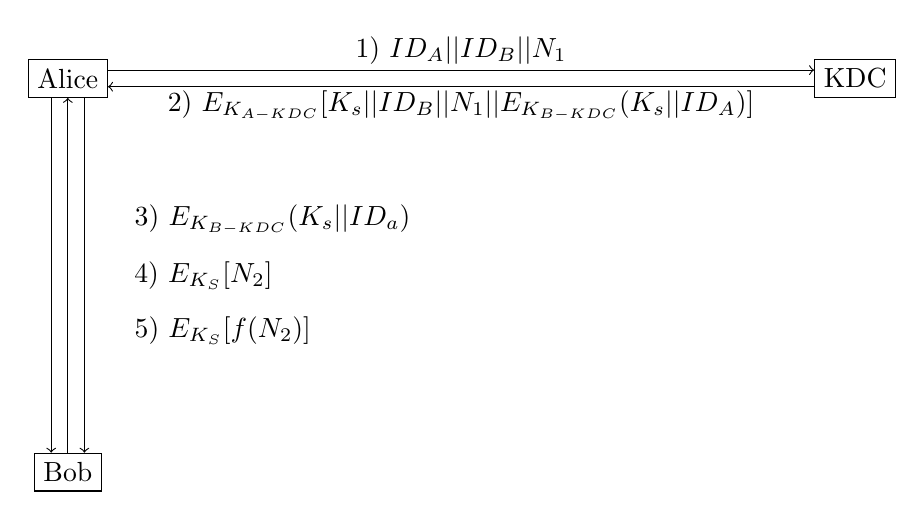
\begin{tikzpicture}
			\node (A) [rectangle, draw=black] at (0, 0) {Alice};
			\node (K) [rectangle, draw=black] at (10, 0) {KDC};
			\node (B) [rectangle, draw=black] at (0, -5) {Bob};

			\draw[->] ([yshift=3pt] A.east) -- node[yshift=7pt]{1) $ID_A || ID_B || N_1$} ([yshift=3pt]  K.west);
			\draw[<-] ([yshift=-3pt] A.east) -- node[yshift=-7pt]{2) $E_{K_{A-KDC}}[K_s || ID_B || N_1 || E_{K_{B-KDC}}(K_s || ID_A) ]$} ([yshift=-3pt]  K.west);

			\draw[->] ([xshift=6pt] A.south) --  node[xshift=68pt, yshift=20pt]{3) $E_{K_{B-KDC}}(K_s || ID_a)$} ([xshift=6pt]  B.north);
			\draw[<-] ([xshift=0pt] A.south) -- node[xshift=49pt, yshift=0pt]{4) $E_{K_{S}}[N_2]$}([xshift=0pt]  B.north);
			\draw[->] ([xshift=-6pt] A.south) -- node[xshift=62pt, yshift=-20pt]{5) $E_{K_{S}}[f(N_2)]$}([xshift=-6pt]  B.north);
		\end{tikzpicture}
		\caption{Basiswerking KDC.}
		\label{fig:basiswerkingKDC}
	\end{figure}
	Een aanvaller kan, indien hij $K_s$ bemachtigd, stap 3 herhalen, zodat de aanvaller nu de Bob zijn response kan beantwoorden. Bob is dan aan het praten met de aanvaller, terwijl hij denkt dat het Alice is.
	Een beter algoritme:
	\begin{enumerate}
		\item Alice informeert Bob dat ze wil communiceren.
		\item Bob antwoordt met een geëncrypteerde nonce $N_2$.
		\item Alice vraagt aan de KDC om communicatie te starten met Bob. Alice verstuurt een andere nonce $N_1$, samen met de geëncrypteerde nonce $N_2$.
		\item De KDC beantwoordt dit met een geëncrypteerd bericht, gebruikmakend van Alice haar sleutel $E_{K_{A-KDC}}$ (De KDC authenticeerd zich op die manier naar Alice toe, en bereikt confidentialiteit). De inhoud van dit is: de sessiesleutel, Bob zijn identiteit, $N_1$, en een geëncrypteerd bericht met de sessiesleutel, $N_2$ en Alice haar identiteit.
		\item Alice verstuurt de sessiesleutel, $N_2$ en haar eigen identiteit geëncrypteerd met de sleutel van Bob naar Bob toe.
		\item Bob antwoordt met een tweede nonce $N_2$, geëncrypteerd met de sessiesleutel, zodat Bob geauthenticeerd is naar Alice toe.
		\item Alice antwoordt terug naar Bob met een bewerkte nonce (een bepaalde functie, bv 1 toevoegen), geëncrypteerd met de sessiesleutel, zodat Alice geauthenticeerd is naar Bob toe.
	\end{enumerate}
	\begin{figure}
		\centering
		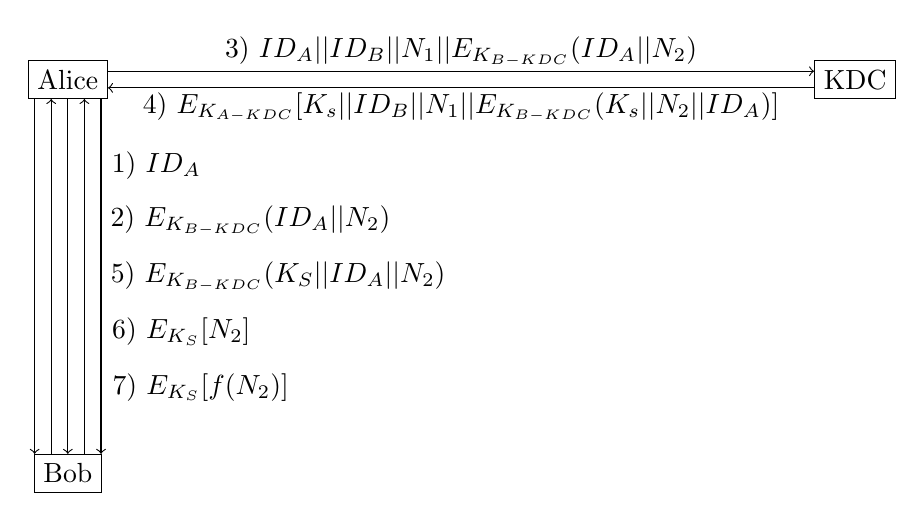
\begin{tikzpicture}
			\node (A) [rectangle, draw=black] at (0, 0) {Alice};
			\node (K) [rectangle, draw=black] at (10, 0) {KDC};
			\node (B) [rectangle, draw=black] at (0, -5) {Bob};

			\draw[->] ([yshift=3pt] A.east) -- node[yshift=7pt]{3) $ID_A || ID_B || N_1 || E_{K_{B-KDC}}(ID_A || N_2)$} ([yshift=3pt]  K.west);
			\draw[<-] ([yshift=-3pt] A.east) -- node[yshift=-7pt]{4) $E_{K_{A-KDC}}[K_s || ID_B || N_1 || E_{K_{B-KDC}}(K_s || N_2 || ID_A) ]$} ([yshift=-3pt]  K.west);

			\draw[->] ([xshift=12pt] A.south)  --  node[xshift=20pt, yshift=40pt]{1) $ID_A$} ([xshift=12pt]  B.north);
			\draw[<-] ([xshift=6pt] A.south)   --  node[xshift=60pt, yshift=20pt]{2) $E_{K_{B-KDC}}(ID_A || N_2)$} ([xshift=6pt]  B.north);
			\draw[->] ([xshift=0pt] A.south)   --  node[xshift=76pt, yshift=0pt]{5) $E_{K_{B-KDC}}(K_S || ID_A || N_2)$} ([xshift=0pt]  B.north);
			\draw[<-] ([xshift=-6pt] A.south)  --  node[xshift=47pt, yshift=-20pt]{6) $E_{K_{S}}[N_2]$} ([xshift=-6pt]  B.north);
			\draw[->] ([xshift=-12pt] A.south) --  node[xshift=60pt, yshift=-40pt]{7) $E_{K_{S}}[f(N_2)]$} ([xshift=-12pt]  B.north);
		\end{tikzpicture}
		\caption{Verbeterde werking KDC.}
		\label{fig:beterewerkingKDC}
	\end{figure}
	\todo{PKI}

	\section{Beveiligen van netwerkprotocollen}
	\subsection{Beveiligen van de transportlaag}
	Het belangrijkste protocol is \textbf{SSL (Secure Socket Layer)}. Het  \textbf{TLS (Transport Layer Security)} protocol is de opvolger van SSL, zodat TLS dus ook alle features heeft van de laatste SSL versie. Hedendaags wordt enkel nog TLS gebruikt.


	In eerste instantie kan SSL/TLS vergeleken worden met SSH, aangezien SSH ook de transportlaag beveiligd. De \underline{verschillen} tussen \underline{SSH} en \underline{SSL/TLS } zijn:
	\begin{itemize}
		\item SSL/TLS  is ontworpen om generiek verkeer over de transportlaag te beveiligen.
		\item SSH bevat ook nog multiplexing, user authenticatie en terminal management. 
		\item SSL gebruikt X.509 certificaten, SSH gebruikt een eigen formaat.
		\item Verschillende optimalisaties: SSH voor shell applicaties en TLS voor betere performantie bij https.
	\end{itemize}

	Verder wordt enkel nog TLS behandelt, SSL kan gegenegeerd worden.

	De \underline{verschillen} tussen \underline{SSH} en \underline{TLS} zijn:
	\begin{itemize}
		\item \textbf{TLS server authenticatie is optioneel.} 
			\begin{itemize}
				\item Anonieme operaties zijn toegelaten.
				\item Hierdoor is een man-in-the-middle attack een zeer eenvoudige aanval.
				\item Server authenticatie in SSH is verplicht.
			\end{itemize}
		\item \textbf{TLS heeft geen user authenticatie.}
			\begin{itemize}
				\item TLS moet enkel de twee interfaces authenticeren (SSH kan dit ook).
				\item User authentication wordt behandeld door een bovenliggende laag.
			\end{itemize}
		\item \textbf{TLS gebruikt X.509 public-key certificaten om te authenticeren.}
			\begin{itemize}
				\item SSH heeft een eigen certificaatformaat.
				\item Vereist een werkend PKI systeem.
				\item Een voordeel van een PKI systeem is dat het schaalbaar is op vlak van sleutelbeheer, iets wat SSH nog niet kan. 
			\end{itemize}
		\item \textbf{TLS kent enkel public-key authenticatie}
			\begin{itemize}
				\item SSH heeft ook nog host-based, password, ...
			\end{itemize}
		\item \textbf{TLS heeft niet de extra features die het SSH connection protocol wel heeft} 
	\end{itemize}

	\subsubsection{Architectuur}
	\begin{itemize}
	\item Een \underline{\textbf{TLS connectie}} is een communicatiekanaal tussen een cliënt en een server. Deze connecties zijn vaak van korte levensduur en servers zullen een connectie zelf vernietigen na een bepaalde tijdsduur indien de connectie te lang op idle modus staat.

	\item Een \underline{\textbf{TLS sessie}} wordt gebruikt om de server een bepaalde staat te geven. De connectie kan gesloten worden, maar kan een sessie behouden. Deze sessie kan dan verdergezet worden met een nieuwe connectie. Een sessie wordt op zowel de client als de server bewaart. Er kan ook een nieuwe sessie aangemaakt worden tijdens een connectie. Een sessie wordt gedefinieerd aan de hand van een aantal parameters:
	\begin{itemize}
		\item De sessieidentifier, een random byte sequentie, gegenereerd door de server.
		\item De optionele X.509 certificaten.
		\item De optionele compressiemethode.
		\item De \emph{master secret}, een gedeelde sleutel van 48 bytes die gekend is door de cliënt en de server.
		\item Een bit \emph{is resumable}, die aangeeft of dat de sessie kan gebruikt worden om nieuwe connecties aan te maken.
	\end{itemize}
	Figuur \ref{fig:two-layer_architecture_TLS} toont aan dat TLS gebruik maakt van een tweelagen architectuur met 
	\begin{enumerate}
		\item het \underline{TLS record layer protocol} en, 
		\item het \underline{TLS-specifieke protocollen}: TLS Handshake protocol, TLS Change Cipher Protocol en TLS Alert Protocol.
	\end{enumerate}
	\begin{figure}[ht]
		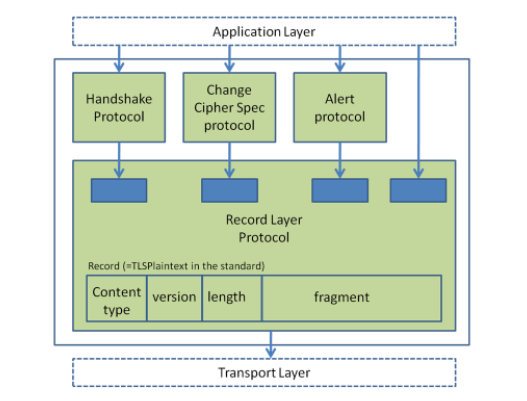
\includegraphics[width=\textwidth]{tls_architecture}
		\caption{Tweelagen architectuur van TLS}
		\label{fig:two-layer_architecture_TLS}
	\end{figure}

	\item Het \underline{\textbf{Handshake protocol}} laat toe om de cliënt en server te authenticeren aan elkaar. Een HP bericht heeft de volgende structuur:
	\begin{itemize}
		\item 1 byte voor de berichtsoort (10 typen gedefinieerd).
		\item 3 bytes voor de berichtgrootte.
		\item variabel aantal bytes voor de eigenlijke informatie, soms zelfs leeg.
	\end{itemize}
	
	Het handshake protocol verloopt in \underline{4} fasen:
	\begin{enumerate}
		\item Eerst moet een TCP sessie aangemaakt worden via het normale TCP process: SYN $\rightarrow$ SYN-ACK $\rightarrow$ ACK.
		\item Daarna verstuurt de clënt een \textbf{client\_hello} bericht naar de server met volgende parameters:
			\begin{itemize}
				\item \textbf{Version}: De hoogste TLS versie waarover de cliënt beschikt.
				\item \textbf{Random}: Een timestamp (32 bits) en 28 bytes gegenereerd door een veilige randomgenerator, dat gebruikt wordt als nonce.
				\item \textbf{SessionID}: Een identifier dat gebruikt wordt om de sessie te identificeren. Wordt onder andere gebruikt om een sessie verder te zetten met een andere connectie.
				\item \textbf{CipherSuite}: Een lijst van combinaties van cryptografische algoritmen die de cliënt ondersteunt. Een combinatie bestaat uit een sleuteluitwisselingsmethode, de encryptiespecificatie, de MAC functie en de pseudorandomfunctie dat gebruikt wordt.
				\item \textbf{CompressionMethod}: Een lijst van compressiemthoden waarover de cliënt beschikt.
			\end{itemize}
			De server reageert met een \textbf{server\_hello} bericht die dezelfde structuur bevat als de client\_hello variant. De server neemt uiteraard de versie en cryptografische algoritmen dat hijzelf ook ondersteund.
		\item Indien authenticatie vereist is, stuurt de server een X.509 certificaat naar de cliënt. \textbf{Optioneel} zal de server ook een certificaat vragen aan de cliënt, indien authenticatie vereist is. De server eindigt met een \textbf{server\_done} bericht. De cliënt antwoordt dan indien nodig met zijn certificaat. De cliënt stuurt ook een \textbf{client\_key\_exchange} bericht, met de nodige informatie om een sessiesleutel te genereren. 
		\item De cliënt verstuurt nu een \textbf{change\_cipher\_spec} bericht (met het Change Cipher Protocol), die de juiste combinatie van cryptografische algoritmen bevat. Tot slot stuurt de cliënt een \textbf{finished} bericht. De server verstuurt dezelfde berichten naar de cliënt. Nu zijn de cliënt en server in staat om te communiceren met elkaar via het SSL Record protocol.
	\end{enumerate}

	\item Het \underline{\textbf{Change Cipher protocol}} kan slechts één bericht verstaan: 1 byte met 1 waarde. Het zorgt ervoor dat de tijdelijke keuze van cryptografische algoritmen de werkelijke keuze wordt. Het kan ook gebruikt worden om de encryptiealgoritmen te veranderen gedurende een connectie.

	\item Het \underline{\textbf{Alert protocol}} bevat berichten met foutmeldingen en waarchuwingen. Een bericht bestaat enerzijds uit één byte, die "fatal" of "warning" aangeeft, en een andere byte die meer uitleg geeft over de fout. 
	
	Mogelijke waarschuwingen:
	\begin{itemize}
		\item Problemen met certificaten.
		\item De connectie wordt verbroken door één van de partijen.
	\end{itemize}
	Mogelijke fouten:
	\begin{itemize}
		\item Problemen met het decompresseren.
		\item Een fout tijdens het handshake protocol (geen geldige beveiligingsparameters gevonden).
		\item Fout ingevulde parameters tijdens het handshake protocol.
	\end{itemize}
	\item Het \underline{\textbf{Record protocol}} is een gelaagd protocol dat informatie zo zal bewerken dat: het bruikbare blokken worden van ten hoogste $2^{14}$ bytes, optioneel de informatie zal compresseren, een MAC zal toevoegen voor integriteit, de informatie zal encrypteren en het resultaat doorsturen. Ontvangen data wordt dan in omgekeerde volgorde bewerkt. De typische workflow gaat als volgt (figuur \ref{fig:tls_record_protocol}):
		\begin{figure}[ht]
			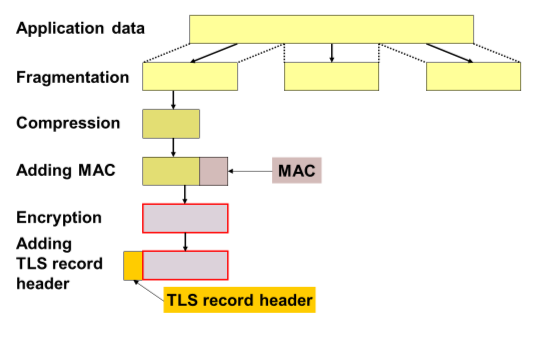
\includegraphics[width=\textwidth]{tls_record_protocol}
			\caption{Werking van het TLS record protocol.}
			\label{fig:tls_record_protocol}
		\end{figure}
		\begin{enumerate}
			\item De informatie wordt verdeeld in fragmenten van hoogstens $2^{14}$ bytes ($\equiv 16$ KB).
			\item De informatie wordt eventueel gecompresseerd. De compressie is optioneel, moet terugkeerbaar zijn, en mag de lengte van de data niet meer dan $1024$ bytes vergroten.
			\item De MAC wordt als volgt berekend: MAC($K_{MAC} || Seq \# || Type || Length || Data$).
			\item De informatie wordt geëncrypteerd met een \underline{symmetrisch encryptiealgoritme}.
			\item De TLS record header wordt toegevoegd. 
		\end{enumerate}
	Het \underline{verschil} met \underline{SSH}:
		\begin{itemize}
			\item SSH zal eerst encrypteren, en dan pas de MAC toevoegen. Geen van beide methoden is beter dan de andere, en komt met zijn eigen problemen.
		\end{itemize}
	De TLS record header heeft volgende structuur (figuur \ref{fig:tls_record_header}):
	\begin{figure}[ht]
		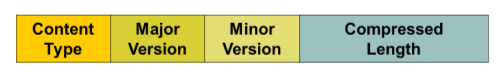
\includegraphics[width=\textwidth]{tls_record_header}
		\caption{De TLS record header.}
		\label{fig:tls_record_header}
	\end{figure}
	\begin{itemize}
		\item 1 byte voor het contenttype. Dit is het applicatielaagprotocol dat gebruikt wordt.
		\item 2 bytes voor de versie (voor TLS 1.2 heeft dit de waarden 3 en 3).
		\item Lengte van de data.
	\end{itemize}

	\item De \underline{\textbf{master secret}}, die nodig is bij een TLS sessie, wordt ofwel gegenereerd door de cliënt met RSA encryptie en verzonden naar de server, ofwel uitgewisseld met Diffie-Helman. De grootte van de sleutel bedraagt 384 bits. Sleutels kunnen niet hergebruikt worden aangezien ze afhankelijk zijn van de nonces die gebruikt werden tijdens het handshake protocol.
	\item Het \underline{\textbf{heartbeat protocol}} draait bovenop het record protocol en heeft voornamelijk als doel om huidige connecties te testen, en om ze in leven te houden zonder dat er opnieuw moet onderhandeld worden tussen de cliënt en de server. Het protocol ondersteund twee berichten:
		\begin{itemize}
			\item \textbf{HeartbeatRequest}: De cliënt of server verstuurt naar de ander een bericht met daarin een payload (typisch een string) en de lengte van de payload. 
			\item \textbf{HeartbeatResponse}: Een ontvanger van een HeartbeatRequest moet antwoorden met dezelfde payload als een HeartbeatResponse.
		\end{itemize}
		\todo{P20 printout C03c}
\end{itemize}

	\subsection{Beveiligen van de netwerklaag}

	\subsection{Beveiligen van de datalinklaag}
	\chapter{Encryptiealgoritmen}
	\section{Geschiedenis}
	Encryptiemethoden worden al eeuwenlang gebruikt om informatie onleesbaar te maken voor partijen die deze informatie niet mogen achterhalen. Deze inleiding bespreekt de basismethoden om encryptie toe te passen.
	
	Zogenaamde \textbf{substitution ciphers} zijn de meest eenvoudigste vorm van encryptie. De originele versie, ook wel \underline{Caesar cipher} genoemd, vervangt elke letter van het alfabet met een voorgedefinieerde shift in positie. Een shift van 3 zal het originele alfabet (in kleine letters) afbeelden op het verschoven alfabet (in grote letters):
	\begin{table}[ht]
	\centering
	\setlength\tabcolsep{1pt}
	\begin{tabular}{c c c c c c c c c c c c c c c c c c c c c c c c c c c}
		a&b&c&d&e&f&g&h&i&j&k&l&m&n&o&p&q&r&s&t&u&v&w&x&y&z \\
		D&E&F&G&H&I&J&K&L&M&N&O&P&Q&R&S&T&U&V&W&X&Y&Z&A&B&C
	\end{tabular}
	\end{table}
	Het duidelijke nadeel is dat er slechts 25 verschillende encryptiemogelijkheden zijn. Een verbeterde versie mapt elke letter met een willekeurige andere (nog niet gebruikte) letter:
		\begin{table}[ht]
		\centering
		\setlength\tabcolsep{1pt}
		\begin{tabular}{c c c c c c c c c c c c c c c c c c c c c c c c c c c}
			a&b&c&d&e&f&g&h&i&j&k&l&m&n&o&p&q&r&s&t&u&v&w&x&y&z \\
			D&K&V&Q&F&I&B&J&W&P&E&S&C&X&H&T&M&Y&A&U&O&L&R&G&Z&N
		\end{tabular}
	\end{table}
	waardoor er nu $26! \approx 4\cdot10^{26}$ mogelijkheden zijn. Deze manier is daarom niet meer secuur, aangezien de onderliggende frequentie van letters nog steeds dezelfde is. Een eenvoudige dencryptiemethode is om de relatieve frequenties van de ciphertekst te tellen, waardoor er statistisch kan achterhaald worden met welke gedecrypteerde letter elke geëncrypteerde letter overeenkomt. 

	Een encryptiealgoritme wil ook de relatieve frequenties verbergen. Een methode dat dit implementeert is de \underline{Vigenère Cipher}. Deze bevat een sleutel $K = k_1k_2 ... k_d$ waarbij $k_i$ het $i$-de alfabet specifieert dat gebruikt moet worden. Na $d$ letters start ment terug vanaf $k_i$.

	Een laatste voorbeeld van een substitutiecipher is de \underline{Playfair cipher}. Hier wordt er een $5x5$ matrix opgesteld, waarbij eerst het sleutelwoord ingevuld wordt, gevolgd door de niet gebruikte letters in alfabetische volgorde. Dit wordt uitgewerkt met de sleutel \texttt{MONARCHY} in Tabel \ref{table:playfair}.
	\begin{table}[ht]
		\centering
		\begin{tabular}{| c | c | c | c | c |}
			\hline
			\accentuate{M} & \accentuate{O} & \accentuate{N} & \accentuate{A} & \accentuate{R} \\
			\hline
			\accentuate{C} & \accentuate{H} & \accentuate{Y} & B & D \\
			\hline
			E & F & G & I/J & K \\
			\hline
			L & P & Q & S & T \\
			\hline
			U & V & W & X & Z \\
			\hline
		\end{tabular}
		\caption{Playfair cipher.}
		\label{table:playfair}
	\end{table}
	Een bericht wordt in paren van letters geëncrypteerd. Stel dat we het woord ballon willen encrypteren, de paren letters worden: ba lx lo nx. Er wordt een x toegevoegd indien er twee dezelfde letters achter elkaar komen, en als het eindpaar uit slechts één letter bestaat. Er kunnen zich drie gevallen voordoen bij elk paar:
	\begin{enumerate}
		\item Als beide letters in dezelfde rij voorkomen, wordt elke letter vervangen door de letter die er rechts van ligt:  \accentuate(on $\rightarrow$ na).
		\item Als beide letters in dezelfde kolom voorkomen, wordt elke letter vervangen door de letter die er onder van ligt: \accentuate(ba $\rightarrow$ ib).
		\item Anders wordt elke letter vervangen door de letter van de kolom van de andere letter: \accentuate(lx $\rightarrow$ su).
	\end{enumerate}
	Er zijn $26 * 26 = 676$ mogelijke diagrammen die gemaakt kunnen worden.

	Na de \textbf{substitution ciphers} zijn er ook \textbf{transposition ciphers}. Zulke ciphers gaan letters niet vervangen, maar gaan ze echter verplaatsen. Dit heeft natuurlijk als nadeel dat de relatieve frequentie van de letters behouden wordt. Twee eenvoudige voorbeelden zijn:
	\begin{enumerate}
		\item Keer elke letter om:
			$$\texttt{A SIMPLE EXAMPLE} \rightarrow \texttt{ELPMAXE ELPMIS A}$$
		\item Keer de woordvolgorde om, en elk woord keert ook de lettervolgorde om:
			$$\texttt{A SIMPLE EXAMPLE} \rightarrow \texttt{A ELPMIS ELPMAXE}$$
	\end{enumerate}
	Een iets beter voorbeeld is de \underline{Rail Fence cipher}. Deze heeft als private sleutel het aantal rijen dat gebruikt wordt. Elke letter zal diagonaal geschreven worden, uitgewerkt in Tabel \ref{table:railfence} op de zin \texttt{DEFEND THE EAST WALL}: 
	\begin{table}[ht]
		\centering
		\begin{tabular}{|c|c|c|c|c|c|c|c|c|c|c|c|c|c|c|c|c|c|c|c|}
			\hline
			D & & & & N & & & & E & & & & T & & & & L & & \\
			\hline
			& E & & E & & D & & H & & E & & S & & W & & L & & X & \\
			\hline
			& & F & & & & T & & & & A & & & & A & & & & X \\
			\hline
		\end{tabular}
		\caption{Rail Fence cipher.}
		\label{table:railfence}
	\end{table}
	Geëncrypteerd is dit dus \texttt{DNETLEEDHESWLXFTAAX}.

	De laatste methode die besproken wordt is de \underline{columnar transposition cipher}. Een bericht wordt in rijen geschreven over een bepaald aantal kolommen. Hierna worden de kolommen gesorteerd op basis van de geheime sleutel $K = k_ik_j ... k_n$. Stel $K = k_3k_4k_2k_1k_5k_6k_7$ en plaintext \texttt{ATTACK POSTPONED UNTIL TWO AM}: Op Tabel \ref{table:columnartransposition} wordt deze plaintext uitgeschreven in rijen en kolommen. De ciphertext wordt dan \texttt{TTNAAPTMTSUOAODWCOIXKNLYPETZ}.
	\begin{table}[ht]
		\centering
		\begin{tabular}{|c|c|c|c|c|c|c|}
			\hline
			A & T & T & A & C & K & P \\
			\hline
			O & S & T & P & O & N & E \\
			\hline
			D & U & N & T & I & L & T \\
			\hline
			W & O & A & M & X & X & X \\
			\hline
		\end{tabular}
		\caption{Rail Fence cipher.}
		\label{table:columnartransposition}
	\end{table}

	Uiteindelijk kan men ook de combinatie maken van \textbf{substitution} en \textbf{transposition} ciphers, wat de basis vormt van moderne cryptografie.

	\section{Symmetrische algoritmen}
	Vooraleer er in detail kan ingegaan worden op symmetrische algoritmen, moet eerst de term \textbf{block cipher} besproken worden. Een block cipher wil zeggen dat informatie in blokken zullen verstuurd worden en kan best vergeleken worden met een substitutiecipher, maar dan toegepast op blokken. Een typische blokgrootte varieert van 8 tot 128 bytes en wordt door de meeste algoritmen gebruikt. De \textbf{Feistel Cipher encryptie} vormt de basis van moderne blockciphers en maakt gebruik van twee primitieve encryptieoperaties:
	\begin{itemize}
		\item Substitutie (de S-box)
		\item Permutatie  (de P-box)
	\end{itemize}
	Het Feistel encryptieschema maakt gebruik van $n$ ronden, een functie $F$ en de XOR operator. \todo{slide 36 uitleggen}

	\subsection{DES \& 3-DES}
	\begin{figure}[ht]
	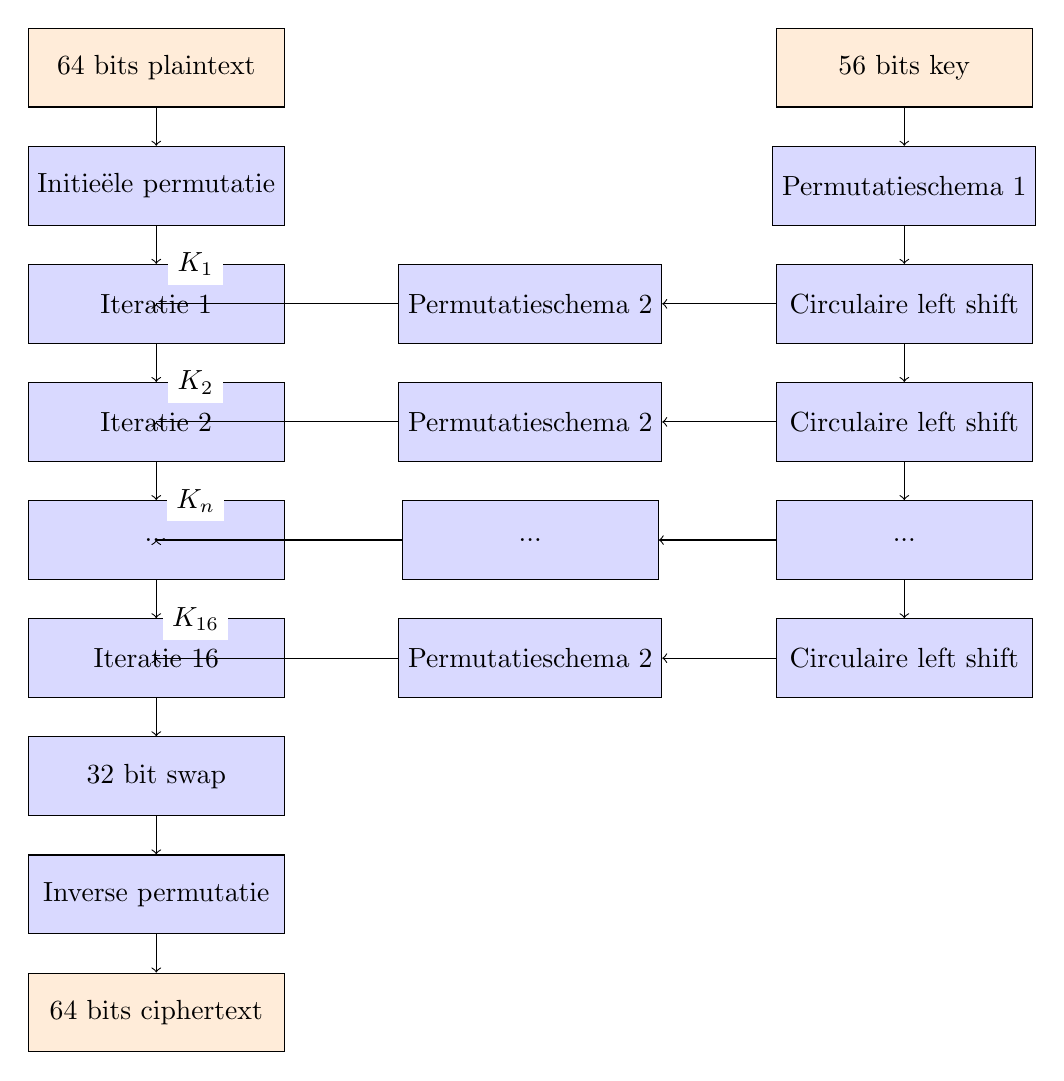
\begin{tikzpicture}[
		base/.style = {rectangle, text centered, draw=black, minimum height=1cm, minimum width=3.25cm},
		orange/.style = {base, fill=orange!15},
		blue/.style = {base, fill=blue!15},
		every node/.style={fill=white, align=center},
		node distance=1.5cm
		]
		\node (plaintext) [orange] {64 bits plaintext};
		\node (IP) [blue, below of=plaintext] {Initieële permutatie};
		\node (it1) [blue, below of=IP] {Iteratie 1};
		\node (it2) [blue, below of=it1] {Iteratie 2};
		\node (itx) [blue, below of=it2] {...};
		\node (it16) [blue, below of=itx] {Iteratie 16};
		\node (bitswap) [blue, below of=it16] {32 bit swap};
		\node (invIP) [blue, below of=bitswap] {Inverse permutatie};

		\node (key) [orange, right of=plaintext, xshift=8cm] {56 bits key};
		\node (PC1) [blue, below of=key] {Permutatieschema 1};
		\node (LCS1) [blue, below of =PC1] {Circulaire left shift};
		\node (LCS2) [blue, below of =LCS1] {Circulaire left shift};
		\node (LCSx) [blue, below of =LCS2] {...};
		\node (LCS16) [blue, below of =LCSx] {Circulaire left shift};

		%PC2x => Permutatieschema 2 voor ronde x
		\node (PC21) [blue, left of= LCS1, xshift=-3.25cm] {Permutatieschema 2};
		\node (PC22) [blue, left of= LCS2, xshift=-3.25cm] {Permutatieschema 2};
		\node (PC2x) [blue, left of= LCSx, xshift=-3.25cm] {...};
		\node (PC216) [blue, left of= LCS16, xshift=-3.25cm] {Permutatieschema 2};

		\node (ciphertext) [orange, below of=invIP] {64 bits ciphertext};

		\draw[->] (plaintext) -- (IP);
		\draw[->] (IP) -- (it1);
		\draw[->] (it1) -- (it2);
		\draw[->] (it2) -- (itx);
		\draw[->] (itx) -- (it16);
		\draw[->] (it16) -- (bitswap);
		\draw[->] (bitswap) -- (invIP);
		\draw[->] (invIP) -- (ciphertext);

		\draw[->] (key) -- (PC1);
		\draw[->] (PC1) -- (LCS1);
		\draw[->] (LCS1) -- (LCS2);
		\draw[->] (LCS2) -- (LCSx);
		\draw[->] (LCSx) -- (LCS16);

		\draw[->] (LCS1) -- (PC21);
		\draw[->] (LCS2) -- (PC22);
		\draw[->] (LCSx) -- (PC2x);
		\draw[->] (LCS16) -- (PC216);

		\draw[->] (PC21) -| node[xshift=0.5cm, yshift=0.5cm]{$K_1$} (it1);
		\draw[->] (PC22) -| node[xshift=0.5cm, yshift=0.5cm]{$K_2$}  (it2);
		\draw[->] (PC2x) -| node[xshift=0.5cm, yshift=0.5cm]{$K_n$}  (itx);
		\draw[->] (PC216) -| node[xshift=0.5cm, yshift=0.5cm]{$K_{16}$}  (it16);

	\end{tikzpicture}
	\caption{DES schema.}
	\label{fig:DES}
\end{figure}

	Het \textbf{DES (Data Encryption Standard)} algoritme maakt gebruik van het reeds vermelde Feistel schema waarbij de \textbf{blokgrootte 64 bits} en \textbf{sleutelgrootte 56 bits} bedraagt. Deze methode is redelijk traag, ondanks de kleine blokgrootte, en wordt door de kleine sleutelgrootte ook als onveilig beschouwd. Een 56 bit sleutel kan namelijk binnen de 10 uur gekraakt worden indien het aantal operatiers per \textbf{micro}seconde $10^6$ bedraagt. 
	
	Het algoritme maakt gebruik van 16 ronden in het Feistel schema. De 56 bit sleutel wordt gebruikt om iteratiesleutels $K_1, K_2, ... K_{16}$ te bepalen, die elk 48 bits groot zijn. Voor de eerste ronde en na de laatste ronde wordt er een extra permutatie uitgevoerd, waarbij de laatste permutatie het inverse is van de eerste permutatie. Het resultaat van dit algoritme is één van de $2^{64}$ uitvoermogelijkheden van de 64 bits. 

	De 16 vereiste iteratiesleutels worden in het begin van het algoritme aangemaakt. Eerst en vooral wordt de 56 bit sleutel gepermuteerd, afhankelijk van het gekozen permutatieschema, op Figuur \ref{fig:DES} permutatieschema 1 genoemd. Een permutatieschema mapt een bit van de oorspronkelijke sleutel op een bit van de gepermuteerde sleutel, zodat er $2^{64}$ mogelijke schemas bestaan. De gepermuteerde sleutel wordt hierna beschouwd als twee resultaatsleutels $C_n$ en $D_n$, met $n$ het huidig rondenummer, van elk 28 bits groot. Beide resultaatsleutels worden onafhankelijk van elkaar verwerkt door een circulaire left shift van 1 of 2 bits, afhankelijk van de huidige ronde, dat eenvoudig door de conditionele operator kan beschreven worden: $n\;\% == 0\;?\;2\;:\;1$. Indien $C_2$ en $D_2$ de resultaatsleutels zijn van ronde 2, dan zijn $C_3$ en $D_3$ de resultaatsleutels van ronde 3 door respectievelijk $C_2$ en $D_2$ 2 bits naar links te permuteren. Voor elke ronde wordt er een iteratiesleutels $K_n$ gegenereerd, door een tweede permutatieschema, op Figuur \ref{fig:DES} permutatieschema 2 genoemd, toe te passen op $C_nD_n$, waarbij de 8 meest significante bits van $C_n$ genegeert worden. Het eindresultaat zijn 16 verschillende iteratiesleutels, die zullen toegepast worden bij elke DES ronde. 

	Bij elke ronde wordt het 64-bit blok opgedeeld in twee 32-bit blokken $L_n$ en $R_n$ waarbij de 32 meest significante bits in $L_n$ komen, en de 32 minst significante bits in $R_n$. Vooraleer dit proces plaatsvindt is er eerst een initiele permutatie van het hele 64-bit blok. Deze permutatie wordt uitgevoerd met behulp van een permutatieschema, zoals bij de sleutelgeneratie. Het gepermuteerde blok wordt hierna opgedeeld in de blokken $L_n$ en $R_n$, en kan ronde 1 van start gaan. Bij elke iteratie wordt de functie $F$ gebruikt, die twee blokken manipuleert: $R_{n-1}$ en de sleutel van 48-bit groot, die op voorhand al gegenereerd werd. Omdat hij elke iteratie wordt gebruikt wordt het ook wel de iteratiefunctie genoemt. De uiteindelijke uitvoer van de iteratiefunctie is een blok 32 bits. $L$ en $R$ kan voor een volgende iteratie berekent worden als:
	\begin{equation}
		\begin{split}
			L_{n + 1} & = R_{n} \\
			R_{n + 1} & = L_{n} \mathbin{\oplus} F(R_{n}, K_{n + 1})
		\end{split}
		\label{formula:DES}
	\end{equation}

	Hoe werkt de iteratiefunctie? Eerst moet het blok $R_n$ uitgebreidt worden via een selectietabel. Het gebruik van deze selectietabel wordt hier voorgesteld als de functie $E(R_n)$, die als input een blok van 32-bit en zal als output een blok van 48-bit genereren waarbij de bits gegroepeerd per 6 zitten. Sommige bits van $R_n$ worden zullen dus meerdere keren gemapt moeten worden. Na deze uitbreiding wordt het resultaat van $E(R_n)$ en de sleutel $K_n$ met een XOR operatie bewerkt (XOR geeft 0 indien beide bits gelijk zijn, en 1 als ze verschillend zijn). Elke groep van 6 bits stelt een adres voor in een welbepaalde substitutie tabel $S_i$, voor de $i$-de groep van 6 bits: er zijn dus 8 substitutietabellen. Elk adres wijst naar een 4-bit getal, dat de originele 6 bits zal vervangen, zodat het eindresultaat terug een blok van 32 bits is. Hoe worden deze 4 bits bepaald? De substitutietabel neemt een blok van 6 bits $B$ als input, de bits $b_5b_4b_3b_2b_1b_0$ van $B$ doen het volgende:
	\begin{itemize}
		\item $b_5$ en $b_0$ representeren tesamen een getal van 0 tot en met 3. Stel dit getal gelijk aan $i$. 
		\item De tussenliggende bits representeren tesamen een getal van 0 tot en met 15. Stel dit getal gelijk aan $j$.
		\item Zoek in de tabel het getal op de $i$-de rij en $j$-de kolom. Dit getal heeft een waarde tussen 0 en 15, en bevat dus slechts 4 bits. Deze bitrepresentatie van dat getal vervangt de 6 bits.
	\end{itemize}
	Tot slot moet er nog een permutatie $P$ uitgevoerd worden op de 32 bits verkregen van de substitutiestap. Met behulp van de iteratiefunctie worden opeenvolgende $L_i$ en $R_i$ bepaalt (formule \ref{formula:DES}).

	\subsubsection{Block cipher modi}
	Er zijn verschillende implementaties van het DES-algoritme, en deze hangen dan weer af van de gebruikte block cipher modus. Verschillende mogelijkheden zijn:
	\begin{itemize}
		\item \textbf{ECB (Electronic Code Book).} Elk 64-bit blok van oorspronkelijke informatie wordt individueel geëncrypteerd
		\item \textbf{CBC (Chain Block Chaning).} Elk cipherblok is nu afhankelijk van elkaar, door een initiële XOR-operatie uit te voeren met het vorige geëncrypteerde blok, en het te encrypteren blok.
		\item \textbf{CFB (Cipher Feedback).} Gelijkaardig aan CBC, maar \todo{wat?}
	\end{itemize}
	\todo{rest van block cipher mody en 3-DES}

	\subsection{AES}
	\todo{no clue what w[x, y] wil zeggen + DECRYPTIE (SLIDE 96)}
	\begin{figure}[ht]
		\begin{tikzpicture}[
			base/.style = {rectangle, text centered, draw=black, minimum height=1cm, minimum width=3.25cm},
			orange/.style = {base, fill=orange!15},
			blue/.style = {base, fill=blue!15},
			every node/.style={fill=white, align=center},
			node distance=1.5cm
			]
			\node (plaintextE) [orange] {128 bits plaintext};
			\node (addkeyE) [blue, below of = plaintextE] {Toevoegen sleutel};
			\node (it1) [blue, below of=addkeyE] {Iteratie 1};
			\node (it2) [blue, below of=it1] {Iteratie 2};
			\node (itx) [blue, below of=it2] {...};
			\node (it10) [blue, below of=itx] {Iteratie 10};

			\node (ciphertextE) [orange, below of =it10] {128 bits ciphertext};

			\draw[->] (plaintext) -- (addkeyE);
			\draw[->] (addkeyE) -- (it1);
			\draw[->] (it1) -- (it2);
			\draw[->] (it2) -- (itx);
			\draw[->] (itx) -- (it10);
			\draw[->] (it10) -- (ciphertextE);

	
		\end{tikzpicture}
		\caption{AES schema.}
		\label{fig:AES}
	\end{figure}

	Het \textbf{AES (Advanced Encryption Standard)} algoritme maakt is ook een symmetrisch encryptiealgoritme waarbij de \textbf{blokgrootte 128 bits} en \textbf{sleutelgrootte 128, 192 of 256 bits} bedraagt. Het werd speciaal ontworpen om cryptoanalyse moeilijk te maken en is zelfs sneller dan 3DES op 32-bit toestellen. Op Figuur \ref{fig:AES} wordt het schema getoond voor een blokgrootte van 128 en een sleutelgrootte van 128 bits. Het schema is gelijkaardig voor een sleutelgrootte van 192 of 256 bits, maar hebben dan respectievelijk 12 en 14 iteraties. Het algoritme is ongeveer 2,5 maal sneller dan het DES algoritme (200 Mbit/s versus 80 Mbit/s) en werkt uitsluitend voor CBC of CTR block cipher modi. Bovendien is het heel goed \textbf{paralleliseerbaar}.

	\section{Asymmetrische algoritmen}
	
	
	\chapter{Software- en systeembeveiliging}
\end{document}